\chapter{Test literature history 16th and 17th century}

\label{ch:exampletest}

This is not the test used as pre- and posttest within the research, but a test provided to the previous generation of students provided by the teacher.

\begin{enumerate}
    \item Provide a Dutch word for the term `renaissance'. Furthermore, explain the central idea of the renaissansistic body of thoughts.
    \item Indicate whether the following statements are `true' or `false':
        \begin{enumerate}
            \item The renaissance originated in the Northern and Central Italian republican citystates.
            \item The literature from the renaissance is only a revival of classical genres.
            \item The eventual goal of renaissance writers is imitatio.
            \item An amount of great playwriters from the renaissance is literarily schooled within a chamber of rhetoric [\emph{rederijkerskamer}].
        \end{enumerate}
    \item What is the essence of humanism?
    \item Read the citation below: [\ldots]
        \begin{enumerate}
            \item What is the title of the book from which this citation originates and who wrote this book?
            \item What was the goal of writing this book and why is the book still attractive to read?
        \end{enumerate}
    \item \begin{enumerate} \item What was the reason for writing the Dutch Authorised Version of the bible [\emph{Statenbijbel}]?
            \item Some of the expressions we are still using come from the Dutch Authorised Version of the bible. Why was this bible, generally stated, so important for language in that time?
        \end{enumerate}
    \item Except of imitatio writers used two other methods. Enlist the three methods in the right order and provide a description for each.
    \item \begin{enumerate} \item Which poet is the great example for those who write lovepoetry in this era? \label{itm:lovepoet}
            \item Explain what platonic love is and what this has to do with lovepoetry from question~\ref{itm:lovepoet} and with the adjoining picture [see figure~\ref{fig:laura}].\label{itm:platoniclove}
        \end{enumerate}
    \item Which combination of terms best displays the central ideas from renaissance literature?
        \begin{enumerate}
            \item Learning and pleasure
            \item Antiquity and church
            \item Love and antiquity
            \item Church and pleasure
        \end{enumerate}
    \item Provide for each of the genres of theater (tragedy, comedy, and farce [\emph{klucht}]) a name of a matching writer and the title of a matching play.
    \item Provide two differences between a tragedy and a farce.
    \item Quickly after Willem-Alexander became king of the Netherlands, he visited different provinces together with M\'{a}xima. The province of Drenthe gave a small book on the occasion of this visit, containing among else the following poem: [\ldots]
        \begin{enumerate}
            \item This poem is a sonnet. Enlist the characteristics of a sonnet regarding the form and content.
            \item Explain how the content-related characteristic is included in the poem above.
            \item Who was our most important sonnet writer in the 17th century?
        \end{enumerate}
    \item \begin{enumerate} \item What is the goal of \emph{emblematiek}? Include the term `analogical thinking' in your answer.
            \item Of which three parts does an emblem exist? Use the original terms/names.
        \end{enumerate}
    \item View and read the emblem below [see figure~\ref{fig:emblem}] and conduct the following assignments:\label{itm:emblem}
        \begin{enumerate}
            \item Explain in your own words which analogy is made in the emblem and which lesson the writer wants to teach the reader.
            \item With which word from the original emblem does the analogy start?
        \end{enumerate}
    \item In the children series `Dappere Dodo', 75 episodes were broadcasted on the Dutch TV between 1955 and 1964. The programm revolved around \emph{Dappere Dodo}, who together with his friends Kees, Uncle Harrie, the captain, Grandfather Buiswater and Mrs Vulpen sailed around the world and experienced all kinds of adventure. `Dodo' is in this series an appropriate name for the main person. Provide a good explanation for this.
    \item The shipsjournal of Bontekoe went up in flames during a shipboard fire. Why did he write the journal again after the sea journey?
    \item What does the Meertens Institute? It occupies itself with:
        \begin{enumerate}
            \item the study and documentation of Dutch language varation and folk culture
            \item research into and documentation of European language and culture
            \item collecting and documenting songs, specific from the period of the 16th and 17th century
            \item research into dialects and socilects in European context.
        \end{enumerate}
\end{enumerate}

\begin{figure}
    \centering
    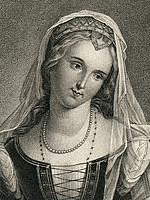
\includegraphics[width=0.3\textwidth]{img/laura.jpg}
    \caption{The figure accompanying question~\protect\ref{itm:platoniclove}}
    \label{fig:laura}
\end{figure}

\begin{figure}
    \centering
    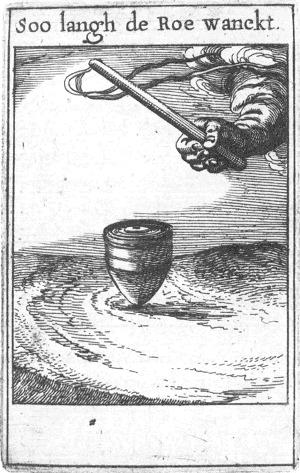
\includegraphics[width=0.3\textwidth]{img/emblem.jpg}
    \caption{The figure accompanying question~\protect\ref{itm:emblem}. This figure was accompanied by the following text: ``Soo lang de Roe wanckt. Veel mesche zijn deughdelijck, soo langh zy onder het kruys en verdruckinghe leven: maer als de Roede van den eers is, soo worden zy luy in den dienste Goods. Ghelijuck enen Drijf-tol, die niet meer gheslaghen of ghegispt en wort, die valt haest in onmacht ende blijft ligghen. Uit: Roemer Visscher, Sinnepoppen.'' In the original test a modern Dutch translation was also provided.}
    \label{fig:emblem}
\end{figure}
